\subsection{PDEBench}
{{\footnotesize
\noindent PDEBench offers forward/inverse PDE tasks with large ready-to-use datasets and baselines (FNO, U-Net, PINN), packaged via a unified API. It won the SimTech Best Paper Award 2023 .


\begin{description}[labelwidth=4cm, labelsep=1em, leftmargin=4cm, itemsep=0.1em, parsep=0em]
  \item[date:] 2022-10-13
  \item[version:] v0.1.0
  \item[last\_updated:] 2025-05
  \item[expired:] unknown
  \item[valid:] yes
  \item[valid\_date:] 2022-10-13
  \item[url:] \href{https://github.com/pdebench/PDEBench}{https://github.com/pdebench/PDEBench}
  \item[doi:] 10.48550/arXiv.2210.07182
  \item[domain:] CFD; Weather Modeling
  \item[focus:] Benchmark suite for ML-based surrogates solving time-dependent PDEs
  \item[keywords:]
    - PDEs
    - CFD
    - scientific ML
    - surrogate modeling
    - NeurIPS
  \item[licensing:] Other
  \item[task\_types:]
    - Supervised Learning
  \item[ai\_capability\_measured:]
    - Time-dependent PDE modeling; physical accuracy
  \item[metrics:]
    - RMSE
    - boundary RMSE
    - Fourier RMSE
  \item[models:]
    - FNO
    - U-Net
    - PINN
    - Gradient-Based inverse methods
  \item[ml\_motif:]
    - Multiple
  \item[type:] Framework
  \item[ml\_task:]
    - Supervised Learning
  \item[solutions:] Solution details are described in the referenced paper or repository.
  \item[notes:] Datasets hosted on DaRUS (DOI:10.18419/darus-2986); contact maintainers by email 

  \item[contact.name:] Makoto Takamoto (makoto.takamoto@neclab.eu)
  \item[contact.email:] unknown
  \item[results.links.name:] ChatGPT LLM
  \item[fair.reproducible:] Yes
  \item[fair.benchmark\_ready:] Yes
  \item[id:] pdebench
  \item[Citations:] \cite{takamoto2024pdebenchextensivebenchmarkscientific}
\end{description}

{\bf Ratings:} ~ \\

\begin{tabular}{p{0.15\textwidth} p{0.07\textwidth} p{0.7\textwidth}}
\hline
Rating & Value & Reason \\
\hline
dataset & 5 & Diverse PDE datasets (synthetic and real-world) hosted on DaRUS with DOIs. Datasets are
well-documented, structured, and follow FAIR practices.
 \\
documentation & 4 & Strong documentation on GitHub including examples, configs, and usage instructions.
Some model-specific details and tutorials could be further expanded.
 \\
metrics & 4 & Includes RMSE, boundary RMSE, and Fourier-domain RMSE. These are well-suited to PDE problems,
though rationale behind metric choices could be expanded in some cases.
 \\
reference\_solution & 4 & Baselines (FNO, U-Net, PINN, etc.) are available and documented, but not every model
includes full training and evaluation reproducibility out-of-the-box.
 \\
software & 5 & GitHub repository (https://github.com/pdebench/PDEBench) is actively maintained and includes
training pipelines, data loaders, and evaluation scripts. Installation and usage are well-documented.
 \\
specification & 5 & Clearly defined tasks for forward and inverse PDE problems, with structured input/output formats,
system constraints, and task specifications.
 \\
\hline
\end{tabular}

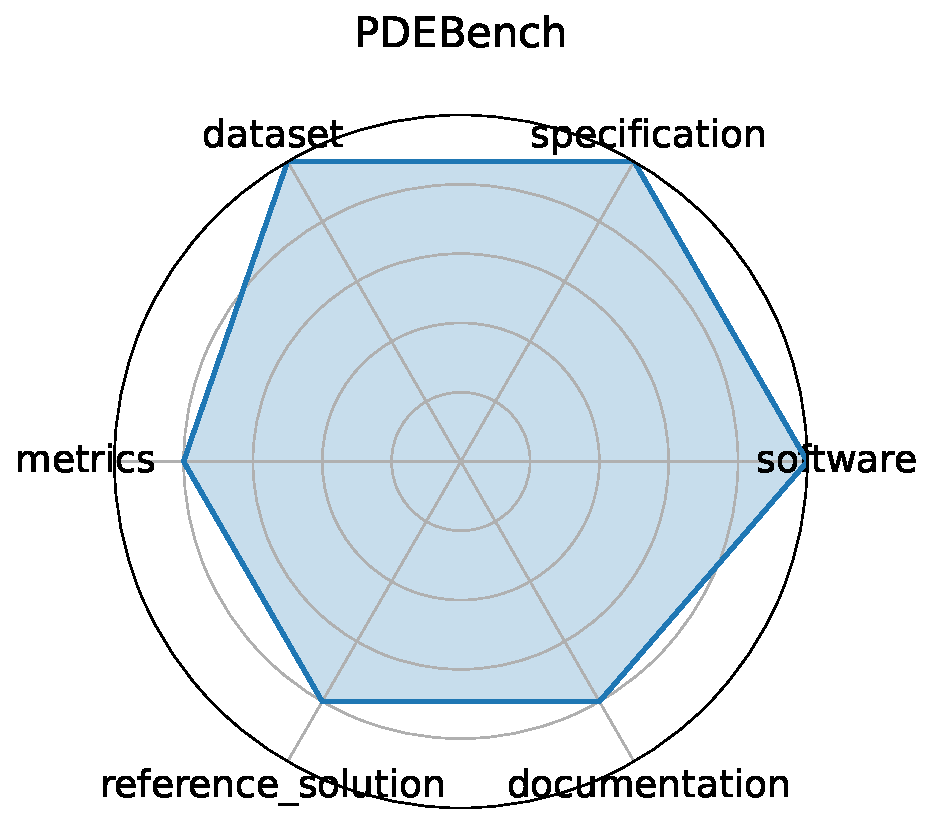
\includegraphics[width=0.2\textwidth]{pdebench_radar.pdf}
}}
\clearpage